\section{Tree Decomposition e programmazione dinamica}

\begin{definition}[Hypergraph]
    Un \emph{hypergraph} è una coppia $H = (V, E)$ dove $V$ è un insieme di \emph{vertici} e $E \subseteq 2^V$ è un insieme di \emph{iper-archi}.

    Un \emph{hyperedge} è un arco che collega più di due vertici.

    \begin{figure}  [H]
        \begin{center}
            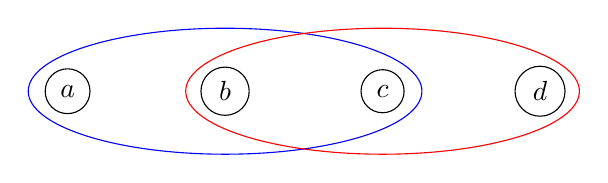
\begin{tikzpicture}
                \draw[color=blue] (2,0) ellipse (2.5 and 0.8);
                \draw[color=red ] (4,0) ellipse (2.5 and 0.8);
                \node[draw, circle] (a) at (0, 0) {$a$};
                \node[draw, circle] (b) at (2, 0) {$b$};
                \node[draw, circle] (c) at (4, 0) {$c$};
                \node[draw, circle] (d) at (6, 0) {$d$};
            \end{tikzpicture}
        \end{center}
    \end{figure}

    Indichiamo con $h$ un iper-arco.

    \begin{itemize}
        \item $h_1 = a,b,c$
        \item $h_2 = b,c,d$
    \end{itemize}

    Possiamo indicare questo con un grafo primale.

    \begin{figure}  [H]
        \begin{center}
            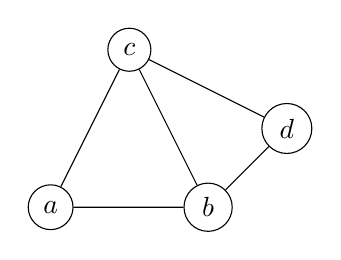
\begin{tikzpicture}
                \node[draw, circle] (a) at (0, 0) {$a$};
                \node[draw, circle] (b) at (2, 0) {$b$};
                \node[draw, circle] (c) at (1, 2) {$c$};
                \node[draw, circle] (d) at (3, 1) {$d$};

                \draw (a) -- (b) -- (c) -- (a);
                \draw (b) -- (d) -- (c);
            \end{tikzpicture}
        \end{center}
    \end{figure}

\end{definition}

\subsection{MIS sui grafi con treewidth limitata}

\textbf{Idea:} Per ogni coppia di bag \textbf{genitore-figlio}, dobbiamo gestire la loro intersezione.

Ad esempio, date due base $B_1= \{B,C,D\}$ e $B_2 = \{C,D,E\}$,
la loro intersezione è $B_1 \cap B_2 = \{C,D\}$. Bisogna risolvere il \textit{sottoproblema} per ogni \textit{sottoinsieme}:
$\{D\}, \{C\}, \{E\}, \{C,D\}, \{C,E\}, \{D,E\}, \{C,D,E\}$.

Diamo qualche definizione di annotazione:

\begin{equation}
    \begin{split}
        \text{La radice} & = R \\
        \text{Una bag} & = X_i \\
        \text{Figlio di $X_i$} & = X_j \\
        \text{Genitore di $X_i$} & = X_{k,i} \\
    \end{split}
\end{equation}

\[
  A[S,i] = MIS(S) \forall S \in X_i + \sum_j MIS(X_j)  
\]

\[
    B[S,i] = \max_{S' \subset X_i} A[S',i], \ \ \ \ S = S' \cap X_{k,i}
\]

\[
    MIS(G) = \max_{S \subset R} B[S,R]
\]


\begin{esempio}
    (Esempio con grafo di prima)
\end{esempio}

\begin{figure}[H]
    \begin{center}
        \begin{tikzpicture}
            %abcdefg
            %a b
            % b - cd
            % c-ef
            %d -fg

            \node[draw, circle] (a) at (4, 0) {$a$};
            \node[draw, circle] (b) at (4, -1) {$b$};
            \node[draw, circle] (c) at (2, -2) {$c$};
            \node[draw, circle] (d) at (6, -2) {$d$};
            \node[draw, circle] (e) at (0, -3) {$e$};
            \node[draw, circle] (f) at (4, -3) {$f$};
            \node[draw, circle] (g) at (8, -3) {$g$};

            \draw (a) -- (b);
            \draw (b) -- (c);
            \draw (b) -- (d);
            \draw (c) -- (f);
            \draw (c) -- (e);
            \draw (d) -- (f);
            \draw (d) -- (g);
        \end{tikzpicture}
    \end{center}
\end{figure}

Riscriviamo le formule cosi:

\begin{equation}
    \begin{aligned}
        A[S,i] &= |S| + \sum_{j} B[S \cap X_{k,i}, j] - |S \cap X_J| \\
        B[S,i] &= \max_{S' \subset X_i} A[S',i]  \ \ \ \ S = S' \cap X_{k,i} \\
    \end{aligned}
\end{equation}

Ora, cerchiamo capire come funziona il tutto.

$B[\mathcal{Z}, i]$.

$\max_{S \subset X_i} Z = S \cap X_{k,i}$.

\begin{itemize}
    \item $\emptyset$ = 0 $\rightarrow$ Z = $\emptyset$
    \item C = 1
    \item E = 1 $\rightarrow$  = $\emptyset$
    \item F = 1
    \item CF = Sono connessi, quindi non calcolo l'IS $- \infty$
    \item CE = Sono connessi, quindi non calcolo l'IS $- \infty$
    \item CEF = Sono connessi, quindi non calcolo l'IS $- \infty$
\end{itemize}

Quindi, praticamente, vediamo l'interseizone diogni sotto insieme con il bag padre, 
e vediamo per quella funzione Z = intersezione bag padre e sottoinsieme contenenti i precedenti indipendent set, prendiamo il valore
di A massimo con la Z che coincide.


Tutto questo SENZA CONSIDERARE LA SOMMATORIA I $A$ perché eravamo nei nodi foglia.
Da ampliare dopo. Commento e poi modifico.

Partiamo dal basso con C E F. Si calcola A di A[empty] = 0, A[C] = A[E] = A[F] = 1. 
Poi B[EMPTY] = 1, B[C] = B[F] = 1.

Poi passa a D F G . Uguale. A[EMPTY] = 0, A[D] = A[F] = A[G] = 1.
Poi B[EMPTY] = 1, B[D] = B[F] = B[D] = 1.

Ora, andiamo a C D F. 
A[EMPTY]. La cardinalità è chiaramento 0. Ora c'è la sommatoria $\sum_{j} B[S \cap X_{k,i}, j] - |S \cap X_J|$. La prima parte è chiaramente B[$\emptyset$] e poi c'è
la sottrazione con la cardinalità di $\emptyset$ che è 0. 
Alla fine avremo $0 + 1 - 0 + 1 - 0$, che è 2.

Vediamo ora $A[C]$. La cardinalità è 1. Ora c'è la sommatoria $\sum_{j} B[S \cap X_{k,i}, j] - |S \cap X_J|$. La prima parte $B[A \cap CEF]$ e la seconda $|S \cap CEF|$.
Ora, c'è un altro figlio e quindi la sommatoria continua con $B[A \cap DFG] - |S \cap DFG|$. Qui l'intersezione è vuota quindi $B[\emptyset]$ = 1 e $|\emptyset|$ = 0. 

La somma finale è: $1 + 1 - 1 +  1 - 0 = 2$.

E si continua ad oltranza.

